\section{Kabel}

\subsection{Reaktanzbelag}
Metallmantel keine Schirmung! Für $D$ nicht $\gg r$!

\textbf{Wechselstromkabel}
\begin{equation*}
    X_{b}' = \pi \left( 4 \ln \left( \frac{D}{r} -1\right) +1 \right) \cdot 10 ^{-2}   \left[\frac{\Omega}{km}\right]
\end{equation*}

\textbf{Einfach-Drehstromkabel}
\begin{equation*}
    X_{b}' = \pi \left( 2 \ln \left( \frac{D_{m}}{r} -1\right) +\frac{1}{2} \right) \cdot 10 ^{-2}   \left[\frac{\Omega}{km}\right]
\end{equation*}

\textbf{Doppel-Drehstromkabel}
\begin{equation*}
    X_{b}' = \pi \left( 2 \ln \left( \frac{D_{m} \cdot D_{L1L\RN{2}}}{r \cdot D_{L1L\RN{1}}} -1\right) +\frac{1}{2} \right) \cdot 10 ^{-2}   \left[\frac{\Omega}{km}\right]
\end{equation*}


\subsection{Suzeptanzbelag}
Metallmantel/-folie schirmt das E-Feld ab !\\
$d =$ Schirmdurchmesser

\textbf{Wechselstromkabel}
\begin{equation*}
    C_{b}' = C_{LE} + 2 \cdot C_{LL} = \frac{\pi \cdot \epsilon_{0} \cdot \epsilon_{r}}{\ln \left( \left(\frac{D}{r}\right) \cdot \frac{(d^2 - D^2)}{(d^2 + D^2)} \right)}
\end{equation*}

\textbf{Einfach-Drehstromkabel}
\begin{equation*}
    C_{b}' = C_{LE} + 3 \cdot C_{LL} = \frac{4 \pi \cdot \epsilon_{0} \cdot \epsilon_{r}}{\ln \left( \left(\frac{D}{r}\right)^2 \cdot \frac{(0,75d^2 - D^2)^3}{(0,75d^2)^3 - (D^2)^3} \right)}
\end{equation*}


\subsection{Konduktanzbelag}
\textcolor{dgreen}{Restleitfähigkeit der Isolierstoffe}
\begin{gather*}
    \tan \delta = \dfrac{I_{R}}{I_{C}} = \dfrac{1}{\omega C R} = \frac{G}{B}\\
    G_{b}' = B_{b}' \cdot \tan \delta = \omega C_{b}' \cdot \tan \delta
\end{gather*}
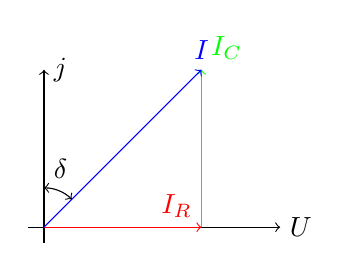
\begin{tikzpicture}
    \draw[->] (-0.2,0) -- (3,0)         node[right] {$\ul{U}$};
    \draw[->] (0,-0.2) -- (0,2)         node[right] {$j$};
    \draw[->, red] (0,0) -- (2,0)       node[above left] {$\ul{I}_{R}$};
    \draw[->, green] (2,0) -- (2,2)     node[above right] {$\ul{I}_{C}$};
    \draw[->, blue] (0,0) -- (2,2)      node[above] {$\ul{I}$};
    \draw[<->] (45:0.5) arc (45:90:0.5) node[above right] {$\delta$};
\end{tikzpicture}


\textbf{Dielektrische Verluste}
\begin{equation*}
    P_{Diel} = \textcolor{red}{(\tan \delta \cdot \epsilon_{r})} \cdot \omega C_{Vakuum} U^2
\end{equation*}

\textcolor{red}{Werkstoff abhängige Verlustziffer}